\subsection{Model Architecture}
\label{sec:arch}


\begin{figure}[!h]
\centering
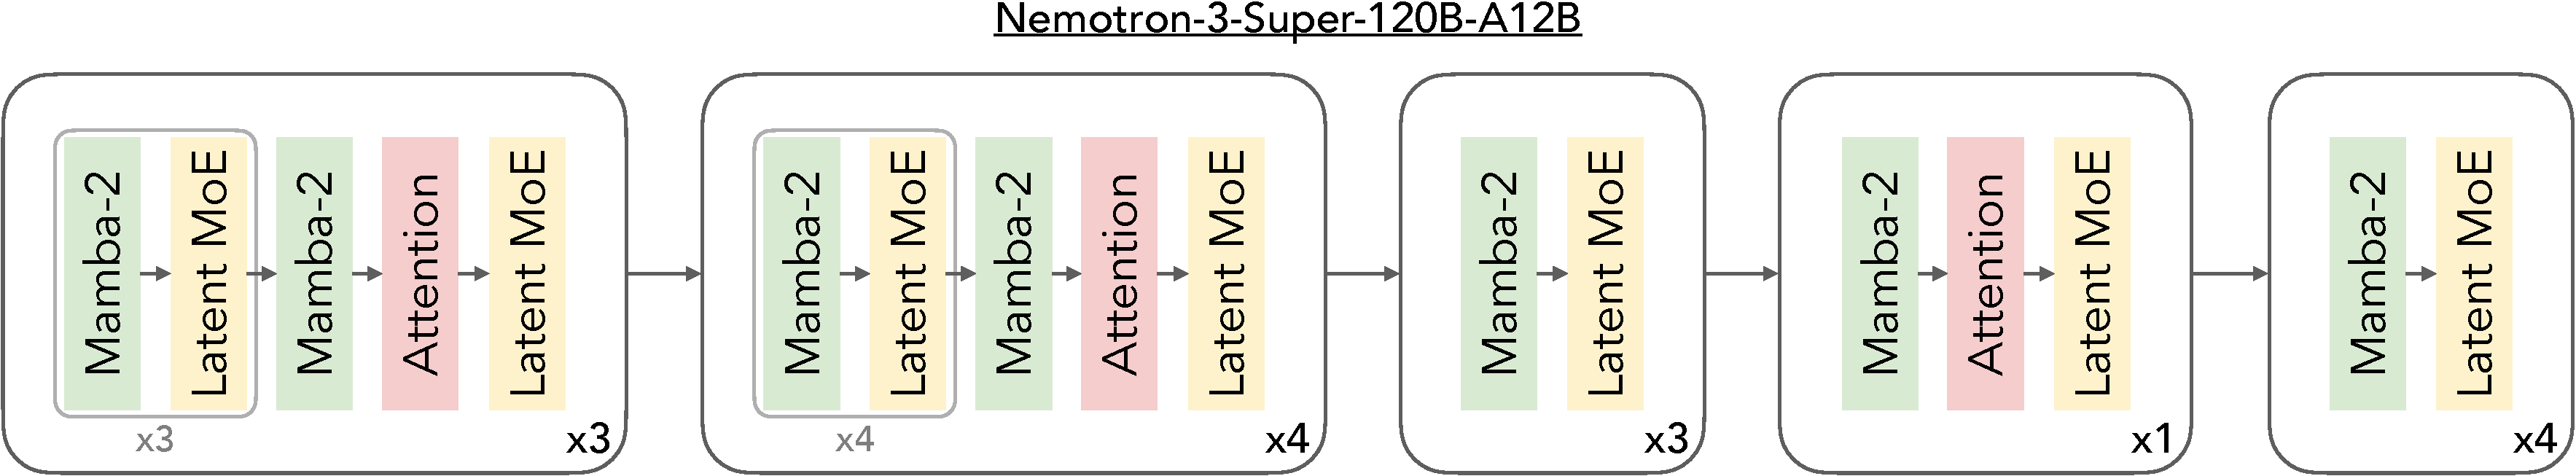
\includegraphics[width=0.9\linewidth]{figures/super-pattern.pdf}
\caption{\ourmodel layer pattern. Similar to \nanomodel, we use a hybrid Mamba-Attention architecture, but \ourmodel is the first model to scale sparsely using LatentMoE layers rather than standard MoE layers.}
\label{fig:layer-pattern}
\end{figure}


\begin{table*}[!hbt]\small\centering
\renewcommand{\arraystretch}{1.2}
\setlength{\tabcolsep}{10pt}
\begin{tabular}{l|c}
\toprule
\textbf{Configuration} & \textbf{\ourbasemodel} \\
\midrule
Total Layers & 88 \\
Model Dimension  & 4096 \\
\midrule
Q-Heads ($n_{q}$) & 32 \\
KV-Heads ($n_{kv}$) & 2 \\
Head Dimension & 128 \\
\midrule
Mamba State Dimension & 128 \\
Mamba Groups & 8  \\ 
Mamba Heads & 128 \\
Mamba Head Dimension & 64 \\ 
\midrule
Expert Hidden Dimension & 2688 \\
Shared Expert Intermediate Size & 5376 \\
Total Experts per Layer & 512 \\
Top-$k$ (Activated Experts) & 22 \\
\midrule
MoE Latent Size & 1024 \\
\midrule
MTP layers (shared weight) & 2 \\ 
\bottomrule
\end{tabular}
\caption{\ourmodel Architectural Dimensions. The model employs a hybrid Mamba-2 and MoE design with strategic global attention layers to optimize the balance between sequence modeling performance and inference throughput.}
\label{table:model_arch}
\end{table*}



\ourbasemodel scales up the hybrid Mamba-Attention Mixture-of-Experts (MoE) architecture introduced in Nemotron-3 Nano~\citep{nvidia2025nvidianemotron3efficient}. We extend this foundation to 120.6B total parameters, maintaining a constrained active budget of 12.7B parameters (12.1B excluding embeddings) per forward pass. The architecture comprises three core pillars: sparse LatentMoE scaling~(\S\ref{sec:latent_moe}), Multi-Token Prediction (MTP) for inference acceleration~(\S\ref{sec:mtp}), and a periodic hybrid interleaving pattern~(\S\ref{sec:hybrid_moe_arch}).


%%%%%%%%%%%%



%\subsubsection{LatentMoE: Hardware-Aware Sparse Scaling}
%To maximize modeling capacity without increasing the inference FLOP budget, \ourbasemodel replaces standard MoE layers with LatentMoE~\citep{latentmoe_tr}. In this framework, input tokens $x \in \mathbb{R}^d$ are projected into a lower-dimensional latent space $\mathbb{R}^l$ ($l=1024$) for routing and expert computation~\citep{latentmoe_tr}. This design yields two primary benefits:
%\begin{itemize}
%    \item \textbf{Efficiency:} It reduces memory bandwidth and all-to-all communication overhead by a factor of $d/l$~\citep{latentmoe_tr}.
%    \item \textbf{Capacity:} These savings allow us to increase the total number of experts to 512 per layer with a Top-22 routing mechanism, significantly improving the accuracy-to-compute ratio.
%\end{itemize}

%The MoE blocks employ squared ReLU activations and a standard MLP router with sigmoid gating and expert biasing~\citep{nvidia2025nemotron3nanoopen}. We additionally utilize two shared experts to further enhance knowledge sharing. 

\subsubsection{LatentMoE: Hardware-Aware Expert Design for Improved Accuracy per Byte} \label{sec:latent_moe}
Mixture-of-Experts (MoE) architectures have emerged as a promising approach to maximize accuracy under fixed inference cost, allowing models to scale in parameter count while keeping floating-point operations (FLOPs) per token constant.
Existing MoE designs are largely motivated by high-level sparsity arguments and optimized for offline, throughput-oriented settings, with little consideration for online deployments that impose strict latency, memory bandwidth, and communication constraints.
Whereas accuracy per FLOP reflects computational efficiency, accuracy per parameter captures memory footprint, memory bandwidth, routing-induced communication, and sharding overhead.
Neglecting these factors can yield architectures that appear efficient in aggregate compute yet incur substantial inefficiency in practice.

Motivated by these observations, we revisited MoE design from a hardware--software co-design perspective.
Through systematic analysis of existing MoE systems across the throughput--latency Pareto frontier, together with accuracy measurements and theoretical analysis, we identified structural inefficiencies in prevailing MoE designs that limit accuracy per unit inference cost.
From this analysis we distilled the following design principles for efficient MoE scaling:
\begin{enumerate}
    \setlength{\itemsep}{0.4em}
    \item In low-latency serving, MoE inference is often dominated by the memory bandwidth cost of reading expert weights. Each expert matrix has size $d \times m$, where $d$ is the hidden dimension and $m$ is the expert FFN intermediate dimension; reducing this cost therefore requires decreasing $d$ or $m$.
    \item In throughput-oriented serving, distributed MoE inference is dominated by all-to-all routing. Routing volume scales as $d \times K$, where $K$ is the number of active experts; reducing communication overhead therefore requires decreasing $d$ or $K$.
    \item Preserving model quality requires preserving the effective nonlinear budget $K \cdot m$. To relieve memory and communication bottlenecks without sacrificing quality, $K$ and $m$ should thus be held fixed.
    \item A task-specific effective feature rank $r_{\mathrm{eff}}$ imposes a lower limit on how much $d$ can be reduced; reducing $d$ below this limit causes model quality to collapse.
    \item Scaling both the total number of experts $N$ and the top-$K$ experts per token improves quality by exponentially expanding the space of expert combinations.
\end{enumerate}
Principles (1)--(3) imply that the hidden dimension $d$ is the most promising axis for reduction, enabling gains in both throughput- and latency-oriented regimes without significant loss in accuracy.
Principle (4) gives a lower bound on how far $d$ can be reduced without collapse.
Principle (5) indicates that increasing $N$ and $K$ improves quality; because memory bandwidth and communication scale linearly with $K$, we can increase $K$ by a factor $\alpha$ and reduce $d$ by the same factor $\alpha$ to obtain higher accuracy at similar inference cost.
Guided by these insights, we developed LatentMoE~\citep{latentmoe_tr}, a MoE architecture designed to achieve higher accuracy than a standard MoE at similar inference cost.


\begin{figure}[h!]
    \centering 
    \begin{subfigure}[t]{0.49\textwidth}
        \centering
        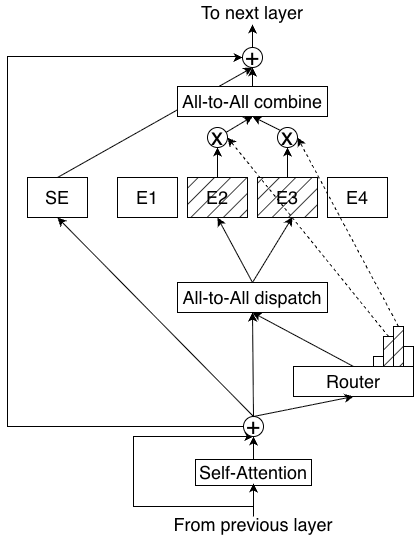
\includegraphics[width=\linewidth]{figures/standard_moe.png}
        \caption{Standard MoE architecture.}
        \label{fig:standard_moe}
    \end{subfigure}
    \hfill
    \begin{subfigure}[t]{0.49\textwidth}
        \centering
        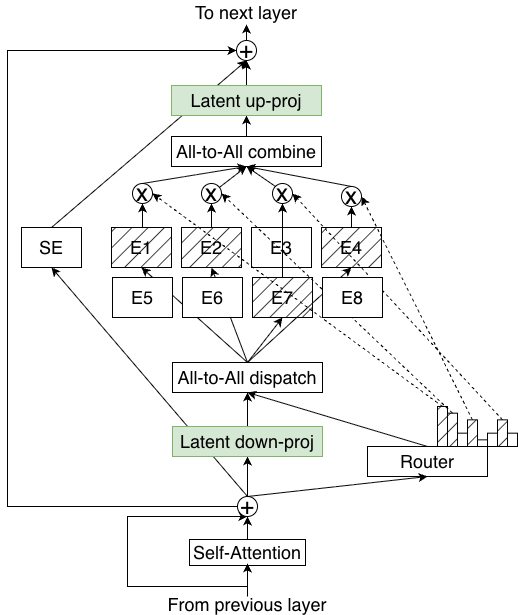
\includegraphics[width=\linewidth]{figures/latent_moe.png}
        \caption{LatentMoE architecture.}
        \label{fig:latent_moe}
    \end{subfigure}
     \caption{Standard MoE vs.\ LatentMoE. In LatentMoE, tokens are projected from the hidden dimension $d$ into a smaller latent dimension $\ell$ for routing and expert computation, reducing routed parameter loads and all-to-all traffic by a factor $d/\ell$. These savings are used to increase both the total number of experts and the top-$K$ active experts per token by the same factor, improving model accuracy at approximately constant inference cost.}
    \label{fig:intro_fig}
\end{figure}


%\begin{figure}[htbp]
%    \centering
%    \begin{subfigure}[b]{0.42\textwidth}
%        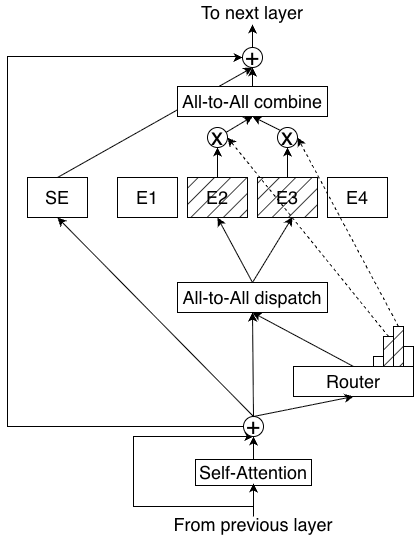
\includegraphics[width=\textwidth]{figures/standard_moe.png}
%        \caption{Standard MoE architecture.}
%        \label{fig:standard_moe}
%    \end{subfigure}
%    \hfill
%    \begin{subfigure}[b]{0.45\textwidth}
%        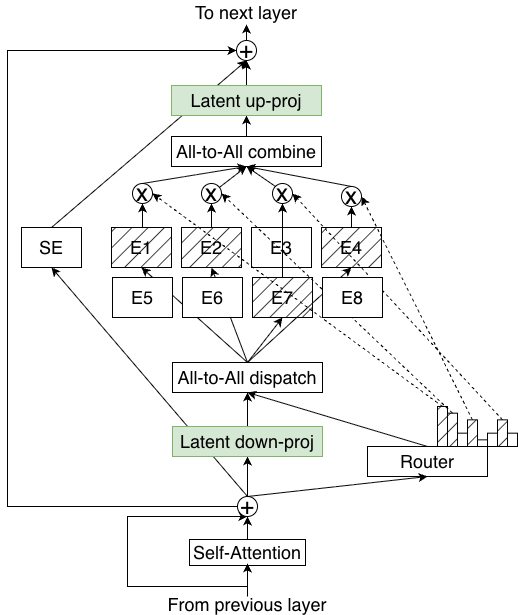
\includegraphics[width=\textwidth]{figures/latent_moe.png}
%        \caption{LatentMoE architecture.}
%        \label{fig:latent_moe}
%    \end{subfigure}
%    \caption{Standard MoE vs.\ LatentMoE. In LatentMoE, tokens are projected from the hidden dimension $d$ into a smaller latent dimension $\ell$ for routing and expert computation, reducing routed parameter loads and all-to-all traffic by a factor $d/\ell$. These savings are used to increase both the total number of experts and the top-$K$ active experts per token by the same factor, improving model accuracy at approximately constant inference cost.}
%    \label{fig:intro_fig}
%\end{figure}

The LatentMoE architecture is illustrated in Figure~\ref{fig:latent_moe}.
Each input token $x \in \mathbb{R}^d$ is first projected into a lower-dimensional latent space $\mathbb{R}^{\ell}$ via a learnable down-projection matrix $W_{\downarrow} \in \mathbb{R}^{\ell \times d}$.
The compressed representation is then routed to an expanded set of experts that operate entirely in this latent space.
After expert computation, the outputs are aggregated and projected back to dimension $d$ via a learnable up-projection matrix $W_{\uparrow} \in \mathbb{R}^{d \times \ell}$.
Shifting routed expert computation and all-to-all traffic into the latent space reduces both per-expert weight loads and communication payloads by a factor $d/\ell$ relative to a standard MoE.
We use these savings to increase the total number of experts from $N$ to $N' = N \cdot d/\ell$ and the top-$K$ active experts per token from $K$ to $K' = K \cdot d/\ell$.
The reduction in dimension offsets the increase in expert count and in $K$, yielding higher model quality at a similar computational and communication budget.
To preserve quality, all non-routed computations---including the routing gate (gating network), shared expert computation, and non-expert layers---remain in the full hidden dimension $d$, as they do not contribute significantly to the targeted bottlenecks.
We refer the reader to the LatentMoE technical report~\citep{latentmoe_tr} for further details.





\subsubsection{Multi-Token Prediction} \label{sec:mtp}
Nemotron-3 Super incorporates a Multi-Token Prediction (MTP) objective to improve both modeling quality and inference efficiency. Unlike conventional next-token training, MTP optimizes the model to predict multiple future tokens at each position~\citep{gloeckle2024better, deepseekai2025deepseekv3technicalreport}. This encourages representations that capture multi-step dependencies and longer-range structure, leading to consistent improvements in validation loss and downstream benchmark accuracy.

Beyond quality gains, MTP enables native speculative decoding. The auxiliary prediction heads function as an internal draft model: during inference, they generate candidate continuations that are verified by the main model in a single forward pass. This substantially reduces decoding latency while introducing minimal additional FLOPs—significantly less than required by an external draft model. Although speculative decoding is particularly effective at small batch sizes, recent work shows that it can also improve throughput in larger-batch and sparse MoE settings~\citep{huang2025moesd}.

\paragraph{Design for Robust Autoregressive Drafting.} Standard MTP implementations use $N$ independent heads, each trained to predict a fixed offset (e.g., $n+2, \dots, n+N+1$). While effective during training, this limits speculative decoding to at most $N$ draft tokens. Longer drafts require either increasing $N$ or reusing a single offset-trained head autoregressively.

Reusing a fixed-offset head introduces a training--inference mismatch: the head is trained under ground-truth hidden states but, at inference, conditions on its own generated states. This distribution shift often reduces acceptance rates as draft length increases.



Nemotron-3 Super addresses this limitation by sharing parameters across multiple MTP heads during training, yielding a unified prediction head exposed to multiple offsets. This shared-weight formulation regularizes the head across prediction horizons and improves robustness to the self-generated hidden states encountered during autoregressive drafting. As a result, the same head can be applied recursively at inference to generate longer drafts with more stable acceptance behavior. While acceptance rates naturally decrease as draft length increases, the degradation is substantially milder than with independently trained offset heads. This enables more effective speculative decoding without introducing additional parameters or requiring a separate draft model.





\paragraph{Speculative Decoding Performance.}
We evaluate MTP quality using SPEED-Bench~\citep{speedbenchnvidia}, a benchmark tailored for speculative decoding. Table~\ref{tab:mtp_speed_bench} reports the average acceptance length (tokens accepted per verification step) with a fixed draft length of 7. Nemotron-3 Super achieves the highest overall average acceptance length (3.45), outperforming DeepSeek-R1 across all domains and remaining competitive with Qwen3-Next.

Figure~\ref{fig:mtp_ar_comparison} plots acceptance rate as a function of draft token index. As expected, acceptance decreases monotonically with draft depth for all models. However, Nemotron-3 Super consistently maintains higher acceptance than DeepSeek-R1 at every draft position and closely tracks or exceeds Qwen3-Next across most indices. Notably, the gap becomes more pronounced at larger draft indices (4–7), where recursive drafting is most challenging. This behavior indicates improved stability of the shared-head autoregressive design under longer speculative rollouts.

Overall, MTP in Nemotron-3 Super improves both representation learning and decoding efficiency, enabling higher acceptance at extended draft lengths without relying on an external draft model. 
These acceptance gains translate to superior serving efficiency on Blackwell hardware. As shown in Figure~\ref{fig:mtp_speed}, increasing the draft depth ($D=1$ to $D=3$) via MTP significantly shifts the throughput--latency Pareto frontier, delivering higher aggregate output tokens per second (TPS) for any given median user latency compared to the baseline with MTP disabled. %\todo{Maor and Izzy please check last paragraph on details of figure 5, please check hardware, ... }

%Nemotron-3 Super addresses this limitation by sharing parameters across multiple MTP heads during training, yielding a unified prediction head exposed to multiple offsets. This shared-weight formulation regularizes the head across prediction horizons, improving robustness to self-generated hidden states encountered during autoregressive drafting. Consequently, the same head can be applied recursively at inference to generate longer drafts without degradation in stability. Empirically, this design maintains high acceptance rates even at extended draft lengths, enabling more effective speculative decoding without introducing additional parameters or requiring a separate draft model.


% While acceptance rates naturally decrease as draft length increases, the degradation is substantially milder than with independently trained offset heads. 

%As a result, the same head can be applied autoregressively at inference to generate longer drafts with more stable acceptance behavior. Although acceptance naturally decreases with draft length (Figure~\ref{fig:mtp_ar_comparison}), the degradation is significantly milder than with independently trained offset heads. This yields consistently higher acceptance at larger draft indices, improving speculative decoding efficiency without additional parameters or a separate draft model.



%Nemotron-3 Super addresses this limitation by sharing parameters across multiple MTP heads during training, effectively learning a unified prediction head that is exposed to multiple offsets. 


%This shared-weight formulation regularizes the head across prediction horizons and makes it inherently robust to recursively generated hidden states.

%This design improves robustness to self-generated hidden states and enables stable autoregressive drafting. As a result, Nemotron-3 Super maintains high acceptance rates even at extended draft lengths without adding extra parameters or a separate draft model.


%This shared-weight formulation regularizes the head across prediction horizons and makes it inherently robust to recursively generated hidden states. At inference, the same head can therefore be applied autoregressively to produce drafts of arbitrary length without degradation in stability.

%Empirically, this design preserves high acceptance rates even at extended draft lengths, enabling more effective speculative decoding without introducing additional parameters or requiring a separate draft model.


%We instead share parameters across MTP heads during training, yielding a unified prediction head exposed to multiple offsets. This design improves robustness to self-generated hidden states and enables stable autoregressive drafting. As a result, Nemotron-3 Super maintains high acceptance rates even at extended draft lengths without adding extra parameters or a separate draft model.

%\paragraph{Design for Robust Autoregressive Drafting.}
%Standard MTP implementations employ $N$ independent heads, each trained to predict a fixed offset (e.g., $n+2, \dots, n+N+1$). This constrains speculative decoding to at most $N$ tokens and limits gains when longer draft lengths are beneficial. Alternatively, some models reuse a single offset-trained head autoregressively at inference time. However, this creates a training–inference mismatch: a head trained for a fixed offset may degrade when recursively applied to its own generated hidden states, reducing acceptance rates.

%To address this limitation, Nemotron-3 Super shares parameters across multiple MTP heads during training, yielding a unified prediction head. This head can be applied autoregressively at inference while remaining robust to distribution shift induced by self-generated hidden states. As a result, the model maintains high acceptance rates even at extended draft lengths, enabling more effective speculative decoding.

%\paragraph{Speculative Decoding Performance.}
%We evaluate MTP quality using SPEED-Bench~\citep{speedbenchnvidia}, a benchmark designed for speculative decoding. Table~\ref{tab:mtp_speed_bench} reports average acceptance length (tokens accepted per verification step) with a fixed draft length of 7. Nemotron-3 Super achieves the highest overall average acceptance length (3.45), outperforming DeepSeek-R1 across all categories and remaining competitive with Qwen3-Next. Figure~\ref{fig:mtp_ar_comparison} further shows that acceptance rates remain stable across draft positions, indicating robustness of the shared-head autoregressive design.

%Overall, MTP in Nemotron-3 Super provides a unified improvement in representation learning and inference efficiency, delivering higher accuracy while enabling low-latency decoding without reliance on an external draft model.

%\ourbasemodel integrates a Multi-Token Prediction objective. Unlike the single-token objective in Nano, MTP enables the model to anticipate multiple future tokens simultaneously~\citep{gloeckle2024better, deepseekai2025deepseekv3technicalreport}. This dual-purpose integration serves to:
%\begin{itemize}
%    \item \textbf{Strengthen Representations:} It encourages the development of internal logic that accounts for multi-step dependencies.
%    \item \textbf{Accelerate Inference:} The MTP layers act as a native speculative decoding engine, generating candidate tokens that can be verified in a single forward pass, thus drastically increasing throughput.
%\end{itemize}

%Multi-Token Prediction (MTP) has emerged as a highly effective technique to improve both the \textit{accuracy} and the \textit{inference efficiency} of large language models. Conventional language model training relies on a next-token prediction loss, however, training for multiple future tokens allows the model to develop better representations for long-range dependencies. Inspired by recent advancements~\citep{gloeckle2024better, deepseekai2025deepseekv3technicalreport}, Nemotron 3 Super is trained to predict multiple future tokens simultaneously at each position.

%For Nemotron-3 Super, this architectural choice serves two primary purposes. First, it yields consistent gains in validation loss and a broad range of downstream benchmarks accuracy. By forcing the model to anticipate future tokens, we encourage the development of internal representations that account for multi-step logic and syntactic structure further down the sequence. 
%Second, MTP allows for seamless speculative decoding synergy. The auxiliary heads effectively act as a built-in draft model. During inference, these heads generate candidate tokens that can be verified by the main model in a single forward pass, drastically reducing latency. MTP introduces minimal additional FLOPs-significantly fewer than required by a separate, external draft model.
%While speculative decoding particularly benefits batch-size-1 scenarios, recent work has shown it can increase throughput across larger batch sizes as well, particularly in sparse MoE architectures \citep{huang2025moesd}.


%Standard MTP implementations typically utilize $N$ independent heads, where each head is trained to predict a specific fixed offset (e.g., $n+2, \dots, n+N+1$). This approach presents a challenge for speculative decoding. Since each head is tied to a specific offset, speculation is limited to $N$ tokens. At lower batch sizes, where inference is often compute-bound, speculation benefits from longer draft lengths than a small fixed number of heads can provide. For instance, Mimo-V2-Flash~\citep{xiao2026mimov2flashtechnicalreport} trained 3 independent MTP heads.
%An alternative approach, seen in models like DeepSeek-R1 and Qwen3-Next~\citep{yang2025qwen3technicalreport}, involves running a single MTP head autoregressively during inference. However, this introduces an inference-training mismatch. A head trained only to predict a specific offset often struggles to maintain high acceptance rates when used recursively, as during inference it encounters its own generated hidden states which may deviate from the training distribution.

%To bridge this gap, Nemotron-3 Super implements parameter sharing across multiple MTP heads during training. This results in a unified head that can effectively be run autoregressively during inference. This design maintains high acceptance rates even for extended draft lengths by ensuring the head is robust to its own generated hidden states.

%We evaluate the accuracy of our MTP implementation using SPEED-Bench~\footnote{https://huggingface.co/datasets/nvidia/SPEED-Bench} ~\citep{speedbenchnvidia}, a dataset curated for speculative decoding evaluation. We compare Nemotron-3 Super against the MTP implementations of Qwen3-Next and DeepSeek-R1.
%Table~\ref{tab:mtp_speed_bench} summarizes the average acceptance lengths (average tokens accepted per step) across various domains in SPEED-Bench using a fixed draft length of 7. Nemotron-3 Super demonstrates a significant lead over DeepSeek-R1 across all categories and remains highly competitive with Qwen3-Next.


\begin{figure}[h!]
    \centering
    
    % Left: Figure
    \begin{minipage}{0.48\textwidth}
        \centering
        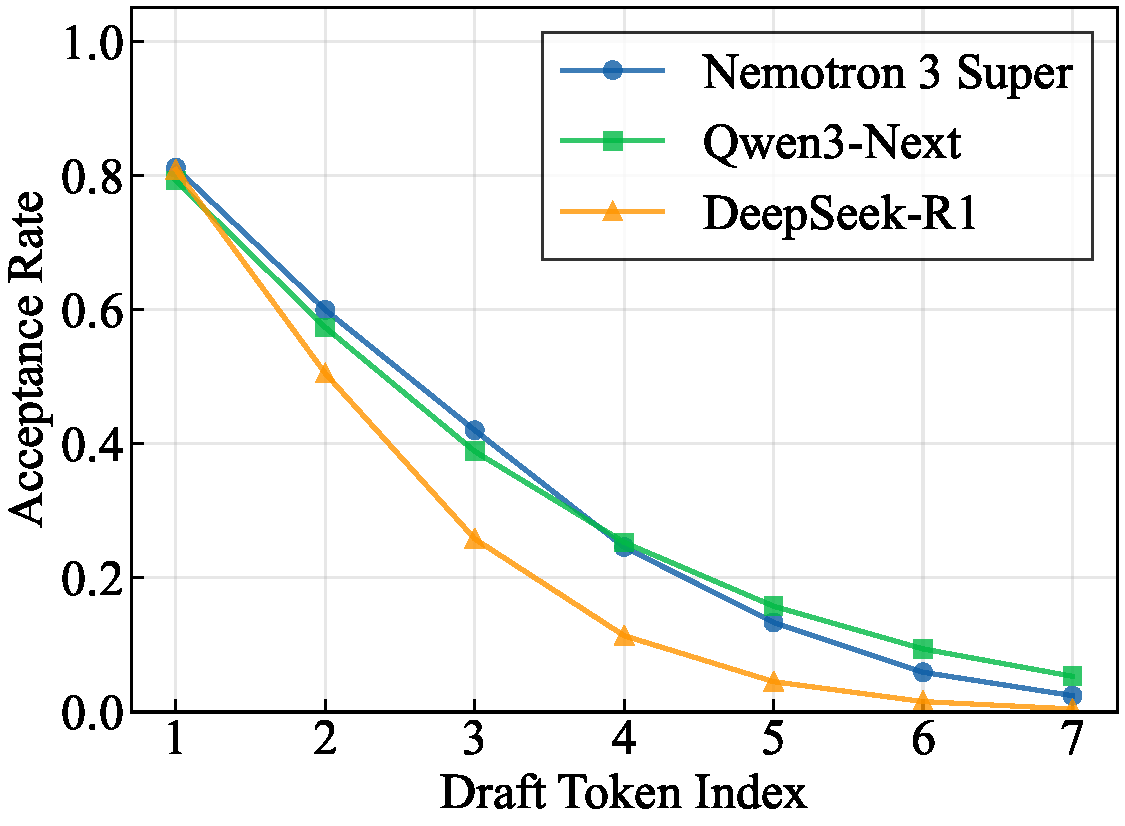
\includegraphics[width=\textwidth]{figures/mtp_ar_comparison_unconditional.pdf}
        \caption{MTP acceptance rate by draft index on SPEED-Bench using a draft length of 7.}
        \label{fig:mtp_ar_comparison}
    \end{minipage}
    \hfill
    % Right: Table (not a float)
    \begin{minipage}{0.48\textwidth}
        \centering
        \footnotesize
        \begin{tabular}{l|ccc}
        \toprule
        \textbf{Category} & \textbf{DSR1} & \textbf{\begin{tabular}[c]{@{}c@{}}Qwen3 \\ Next\end{tabular}} & \textbf{\begin{tabular}[c]{@{}c@{}}Nemotron3 \\ Super\end{tabular}} \\
        %\textbf{Category} & \textbf{DSR1} & \textbf{Q3-Next} & \textbf{N3 Super} \\
        \midrule
        Coding          & 2.99 & \textbf{4.32} & 3.78 \\
        Humanities      & 2.67 & 3.07          & \textbf{3.26} \\
        Math            & 2.98 & \textbf{3.89} & 3.73 \\
        Multilingual    & 2.83 & 3.97 & \textbf{4.05} \\
        QA              & 2.63 & 3.09 & \textbf{3.16} \\
        RAG             & 2.79 & 3.53 & \textbf{3.78} \\
        Reasoning       & 2.80 & 3.47 & \textbf{3.59} \\
        Roleplay        & 2.19 & 2.17          & \textbf{2.82} \\
        STEM            & 2.79 & \textbf{3.37} & 3.30 \\
        Summarization   & 2.59 & 3.06          & \textbf{3.48} \\
        Writing         & 2.41 & 2.69          & \textbf{2.99} \\
        \midrule
        \textbf{Average} & 2.70 & 3.33 & \textbf{3.45} \\
        \bottomrule
        \end{tabular}
        \captionof{table}{MTP average acceptance lengths on SPEED-Bench using a draft length of 7.}
        \label{tab:mtp_speed_bench}
    \end{minipage} \par
    \vskip\floatsep
    \begin{minipage}{0.48\textwidth}
            \centering
        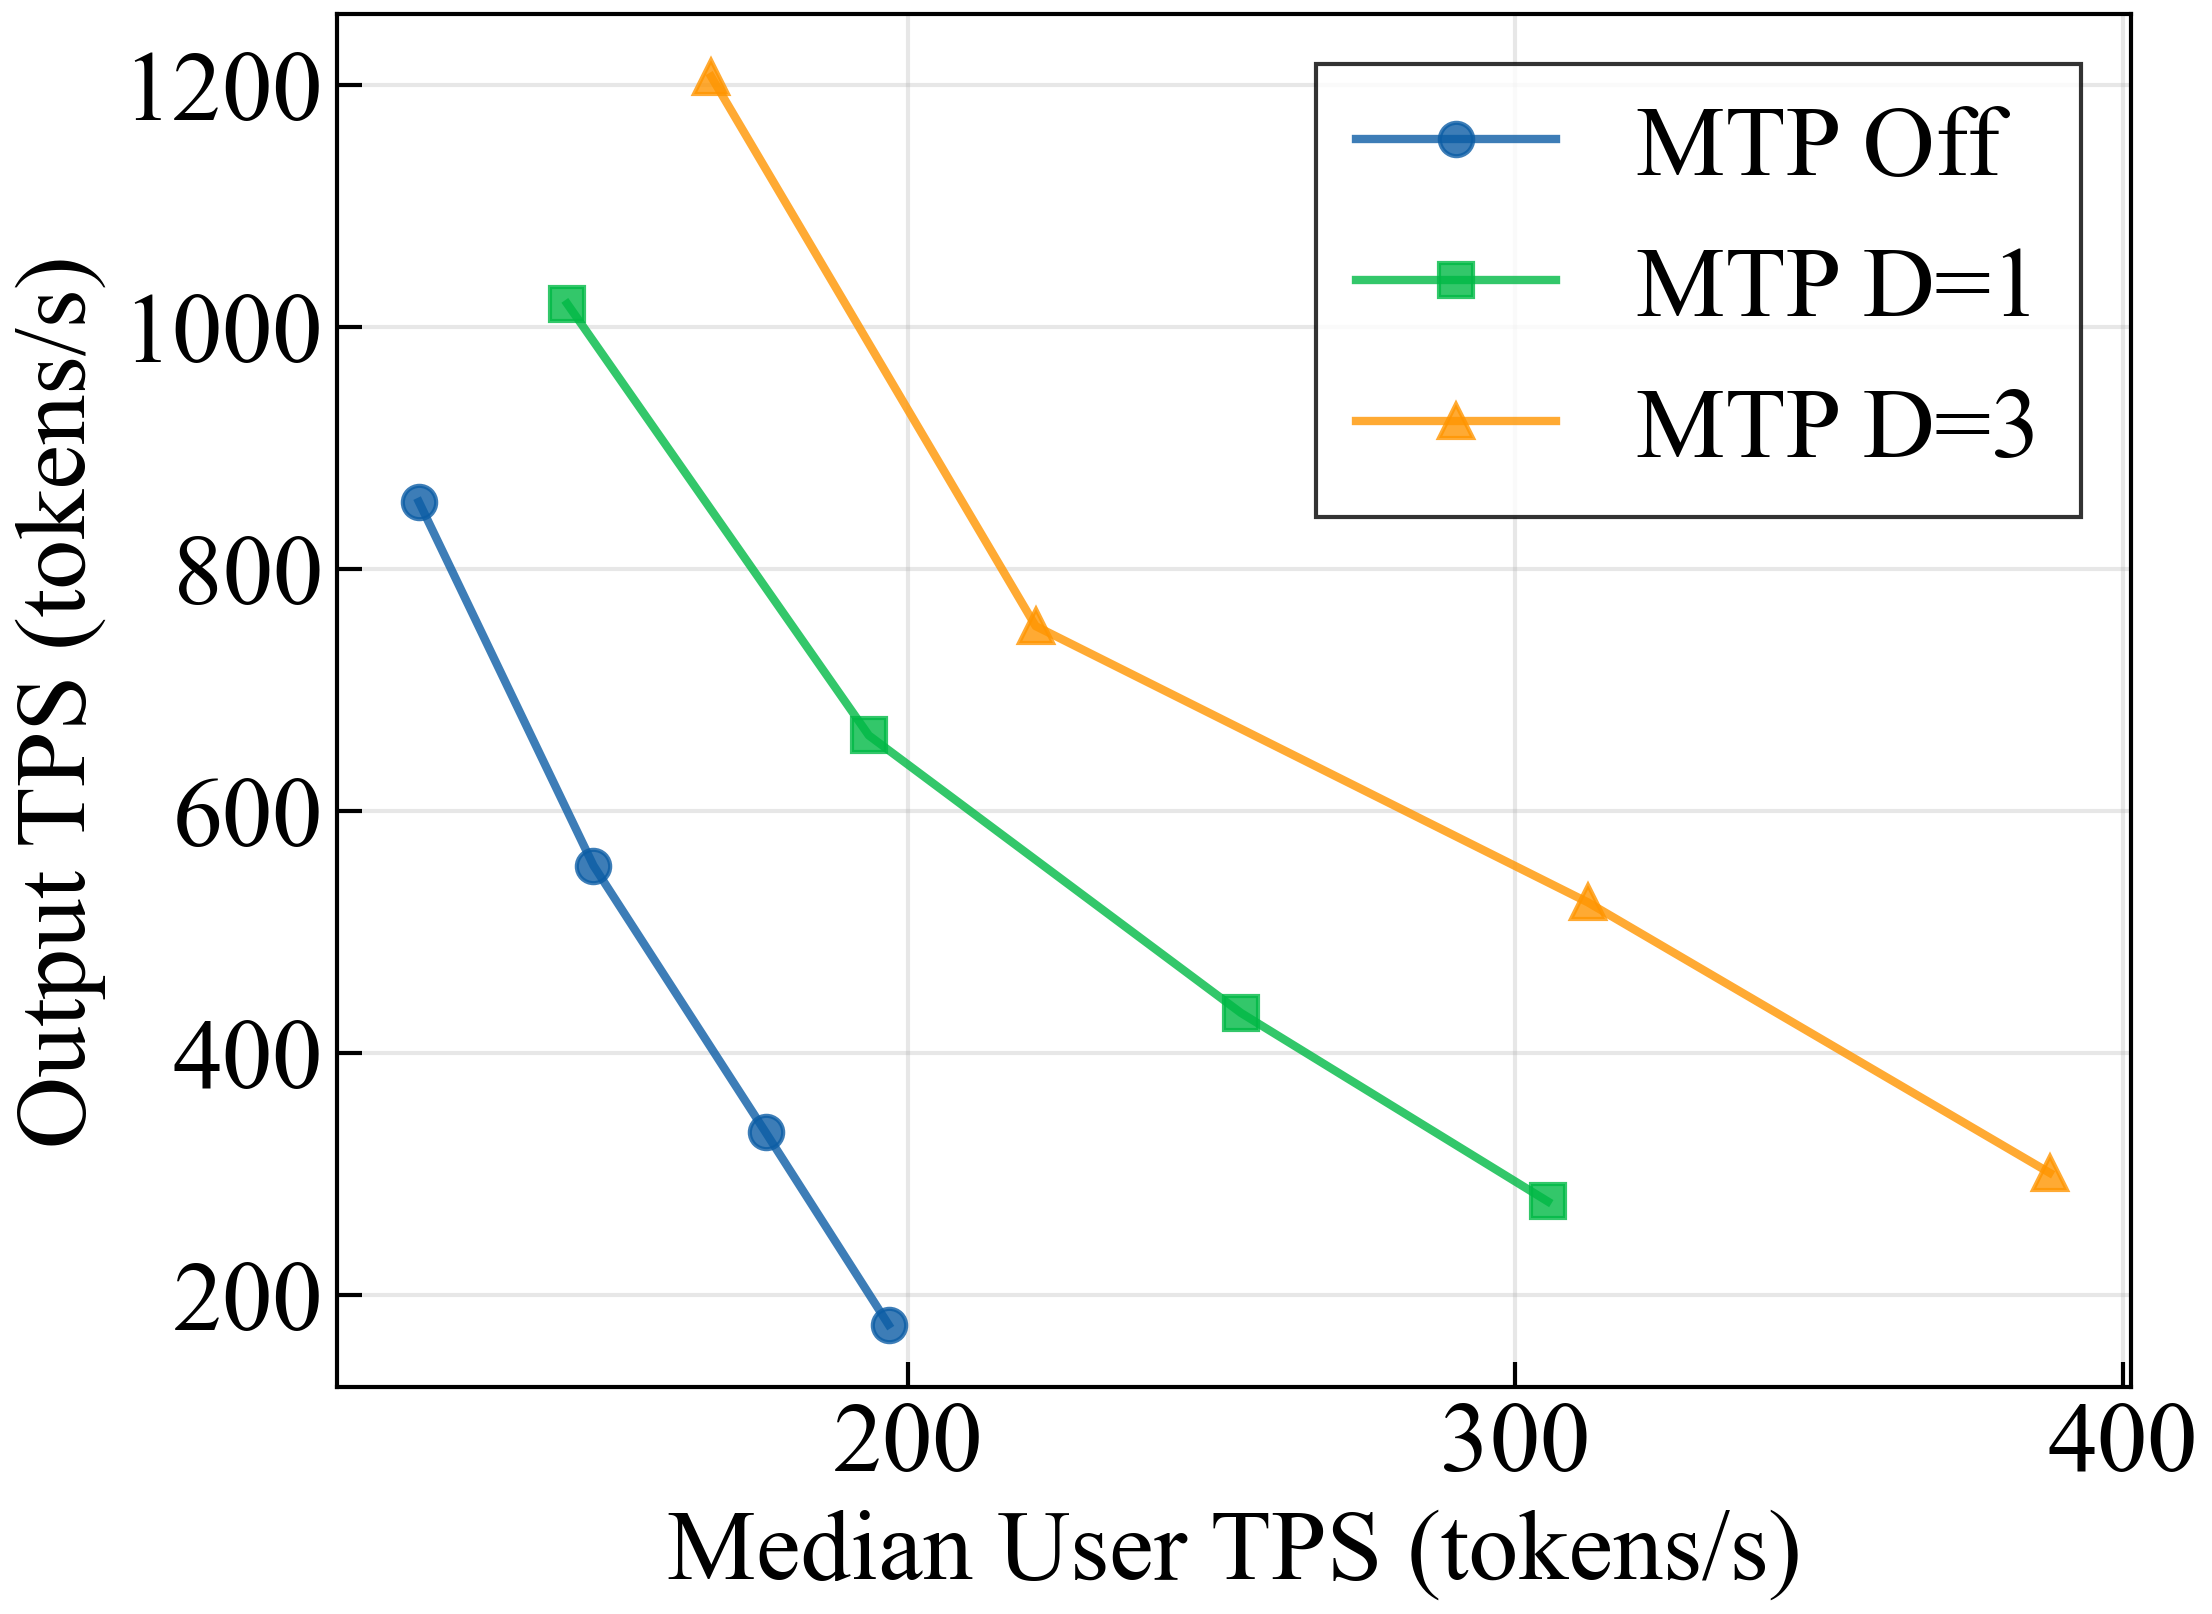
\includegraphics[width=\textwidth]{figures/mtp_trtllm_perf.png}
        \caption{Total vs. user throughput for an NVFP4 checkpoint (TRT-LLM, TP=1, B300 GPU). Comparing MTP off vs. MTP with draft lengths of 1,3. Measured on SPEED-Bench's Throughput-1k split, with 1k output tokens. %NVFP4 Super TRTLLM running SPEED-Bench Throughput\_1k split, TP1 and 1024 max output tokens.
        }
        \label{fig:mtp_speed}
    \end{minipage}
\end{figure}

% \begin{figure}[h!]
%     \centering
%     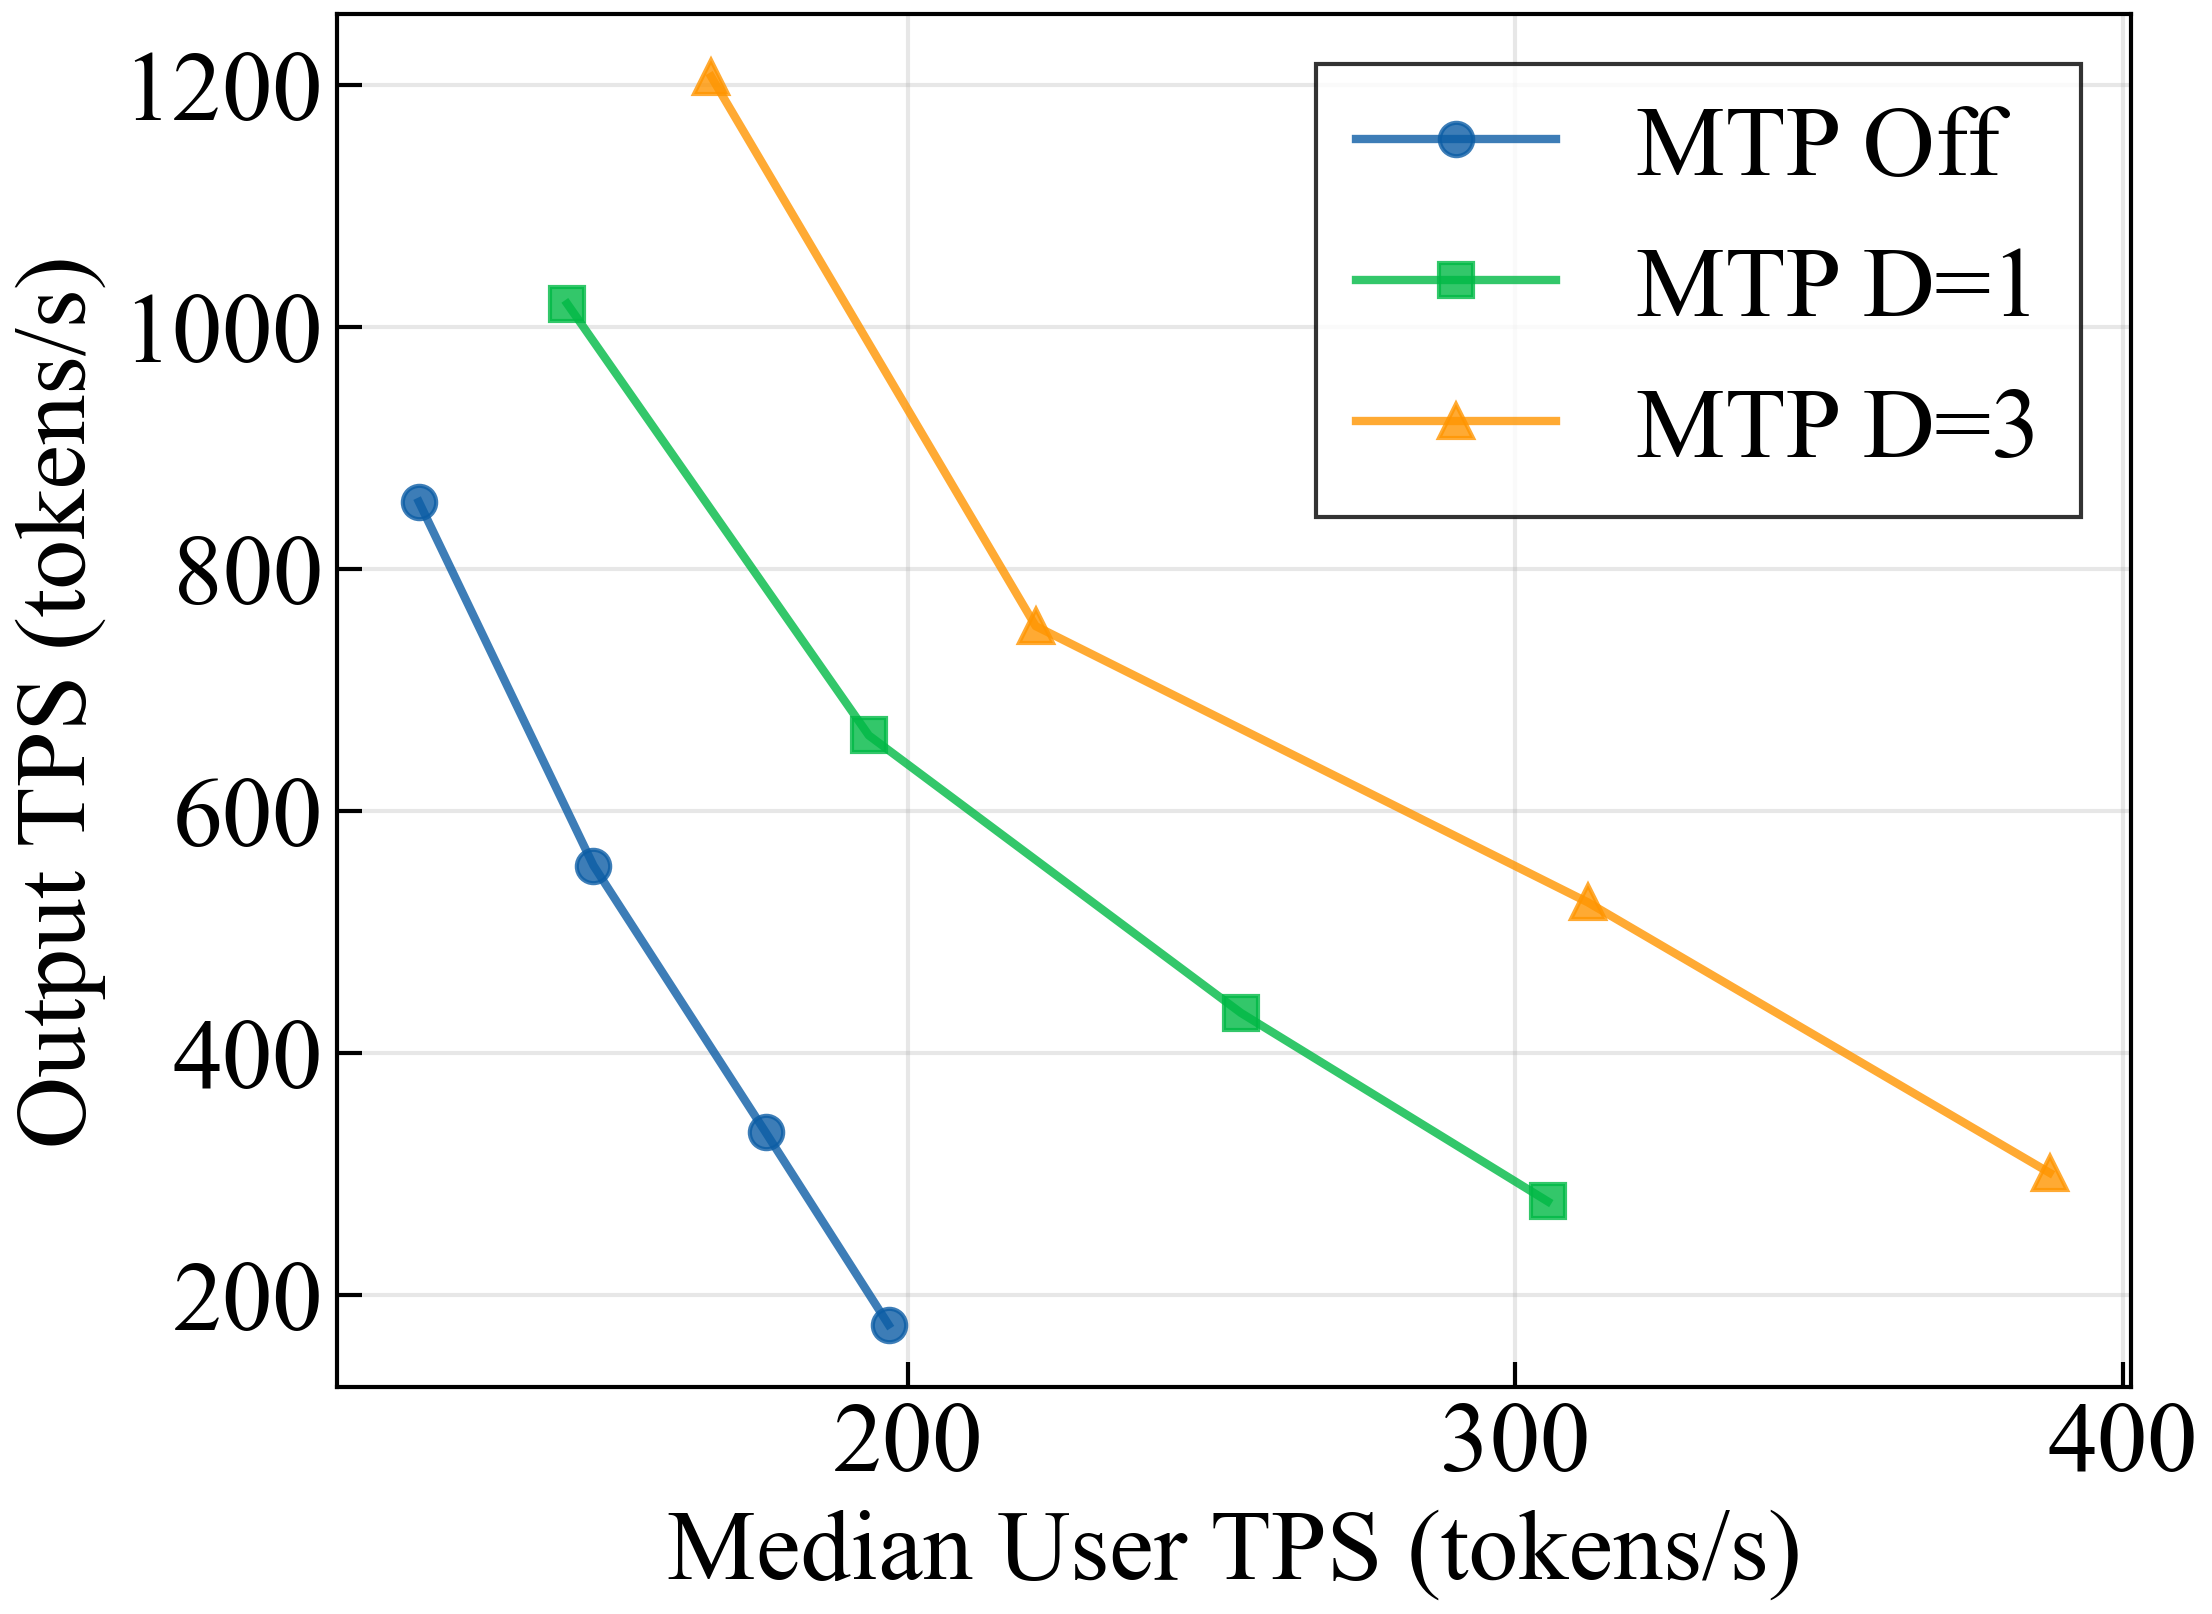
\includegraphics[width=\textwidth]{figures/mtp_trtllm_perf.png}
%     \caption{B300 NVFP4 Super TRTLLM running SPEED-Bench Throughput\_1k split, TP1 and 1024 max output tokens.}
%     \label{fig:mtp_speed}
% \end{figure}
% \begin{table}[h!]
% \centering
% \footnotesize
% \begin{tabular}{l|ccc}
% \toprule
% \textbf{Category} & \textbf{DeepSeek-R1} & \textbf{Qwen3-Next} & \textbf{Nemotron 3 Super} \\
% \midrule
% Coding          & 2.99 & \textbf{4.32} & 3.52 \\
% Humanities      & 2.67 & 3.07          & \textbf{3.16} \\
% Math            & 2.98 & \textbf{3.89} & 3.54 \\
% Multilingual    & 2.83 & \textbf{3.97} & 3.67 \\
% QA              & 2.63 & \textbf{3.09} & 3.06 \\
% RAG             & 2.79 & \textbf{3.53} & 3.50 \\
% Reasoning       & 2.80 & \textbf{3.47} & 3.42 \\
% Roleplay        & 2.19 & 2.17          & \textbf{2.64} \\
% STEM            & 2.79 & \textbf{3.37} & 3.19 \\
% Summarization   & 2.59 & 3.06          & \textbf{3.30} \\
% Writing         & 2.41 & 2.69          & \textbf{2.81} \\
% \midrule
% \textbf{Average} & 2.70 & \textbf{3.33} & 3.25 \\
% \bottomrule
% \end{tabular}
% \caption{MTP average acceptance lengths on SPEED-Bench using a fixed draft length of 7. \textcolor{red}{Note: Results are from the latest RL checkpoint, which did not train the MTP. Before RL, we had an average of 3.6. Continual training should boost these results, so this table should be updated.}}
% \label{tab:mtp_speed_bench}
% \end{table}




\subsubsection{Hybrid Interleaved MoE Architecture and Global Anchors} \label{sec:hybrid_moe_arch}

\ourmodel adopts a hybrid Mixture-of-Experts (MoE) architecture designed to maximize inference throughput—particularly for long-context reasoning—while preserving the modeling capacity of large-scale dense Transformers. The primary systems bottleneck in modern sequence models is the quadratic growth of the KV cache in self-attention layers. To address this, we predominantly utilize Mamba-2 blocks~\citep{dao2024transformersssmsgeneralizedmodels}, which operate with a constant-sized state during generation, substantially reducing memory overhead and latency.

The 88-layer stack follows a periodic interleaving pattern in which MoE layers are paired with Mamba-2 blocks. While Mamba provides efficient linear-time sequence modeling, a limited number of self-attention layers are strategically inserted as global ``anchors'' to enable full-token interaction and long-range information routing across the stack. This hybrid interleaving preserves global dependency modeling while offloading the majority of computation to the more efficient Mamba and sparse MoE components. Table~\ref{table:model_arch} and Figure~\ref{fig:layer-pattern} provide a comprehensive summary of the structural parameters and the specific interleaving pattern of the hybrid stack.

The attention layers employ Grouped-Query Attention (GQA) with 32 query heads and 2 KV heads (head dimension 128). Consistent with prior Nemotron models, we omit positional embeddings, dropout, and bias terms in linear layers, use RMSNorm for normalization, and maintain un-tied embedding and output weights. This configuration supports context lengths of up to 1M tokens.

Sparse scaling further improves efficiency. Each MoE layer activates only a subset of experts per token (top-22 routing), enabling the model to scale to 120.6B total parameters while maintaining a 12.7B active parameter budget per forward pass. %This high capacity-to-compute ratio allows \ourmodel to achieve up to 7.5$\times$ higher inference throughput compared to similarly sized models under common workloads (e.g., 8k input / 64k output). %\todo{Roger, please insert measured throughput and comparison baseline.}

Overall, the synergy between linear-time Mamba blocks, sparsely activated MoE capacity, and strategically placed attention anchors enables \ourmodel to deliver strong long-context performance while remaining optimized for real-world deployment on modern hardware.



%\subsubsection{Hybrid Interleaving and Global Anchors} \label{sec:hybrid-with-anchor}
%The 88-layer hybrid stack follows a periodic interleaving pattern where MoE layers are primarily paired with Mamba-2 blocks. Mamba-2 layers enable efficient sequence modeling with a constant-sized state. To facilitate all-to-all information routing across the stack, we strategically integrate a limited number of self-attention layers as global ``anchors''. 



%The attention layers utilize Grouped-Query Attention (GQA) with 32 query heads and 2 KV heads (128 head dimension). Consistent with the Nemotron family principles, we omit positional embeddings, dropout, and bias terms in linear layers, using RMSNorm for normalization and maintaining un-tied embedding and output weights. This configuration supports ultra-long context lengths of up to 1M tokens. 

%Table~\ref{table:model_arch} and Figure~\ref{fig:layer-pattern} provide a comprehensive summary of the structural parameters and the specific interleaving pattern of the hybrid stack.








%%%%%%%%%%

%\ourbasemodel builds directly upon the hybrid Mamba-Transformer Mixture-of-Experts (MoE) architecture introduced in Nemotron-3 Nano~\citep{nvidia2025nvidianemotron3efficient}. We extend this foundation by scaling the model to 120.6B total parameters (12.7B active per forward pass, 12.1B excluding embeddings) while introducing two critical architectural advancements: \textit{LatentMoE}~\citep{} and Multi-Token Prediction (MTP)~\citep{}

%\subsubsection{Scaling Sparse Capacity with LatentMoE}
%While maintaining the core sparse-scaling philosophy of Nano, \ourbasemodel replaces standard MoE layers with LatentMoE[cite: 8, 38]. This hardware-aware design projects input tokens into a lower-dimensional latent space for expert computation, reducing memory bandwidth and communication overhead[cite: 88, 90]. These efficiency gains allow us to scale the expert pool significantly—utilizing 512 total experts per layer with a Top-22 routing mechanism—thereby improving modeling capacity without increasing the inference FLOP budget[cite: 35, 91, 92].



%\subsubsection{Inference Acceleration via MTP}
%To further optimize the model for agentic deployment, we integrate Multi-Token Prediction (MTP) layers featuring shared weights[cite: 8, 48]. Unlike the standard single-token objective used in Nano, this architectural extension enables \ourbasemodel to anticipate multiple future tokens simultaneously[cite: 132]. This design not only strengthens internal representations for complex reasoning but also serves as a native speculative decoding engine, facilitating significantly higher inference throughput during generation[cite: 135, 137, 138].

%\subsubsection{Hybrid Interleaving and Dimensions}
%The model maintains the periodic interleaving pattern of Mamba-2 blocks and MoE layers, anchored by strategic global attention layers to facilitate all-to-all information routing[cite: 55, 56]. The 88-layer stack utilizes Grouped-Query Attention (GQA) with 32 query heads and 2 KV heads, supporting an ultra-long context length of up to 1M tokens[cite: 10, 35, 36, 49].

%\subsection{Model Architecture}
%\ourbasemodel evolves the hybrid Mamba-Transformer design of Nemotron-3 Nano~\citep{nvidia2025nvidianemotron3efficient} by integrating a sparse Mixture-of-Experts (MoE) framework to maximize accuracy within a constrained active parameter budget~\citep{shazeer2017outrageously, nvidia2025nvidianemotron3efficient}. This architecture is further distinguished by the inclusion of \textit{LatentMoE} for hardware-aware efficiency and Multi-Token Prediction (MTP) for enhanced representation learning and inference acceleration[cite: 8, 48].

%The model comprises 120.6B total parameters, with 12.7B active per forward pass (12.1B excluding embeddings)[cite: 39]. To optimize modeling capacity, we employ a granular MoE structure utilizing shared experts~\citep{dai2024deepseekmoe} alongside a specialized MoE latent architecture[cite: 40, 41]. 

%\subsubsection{LatentMoE and MTP Integration}
%The core innovation in \ourbasemodel is the transition to LatentMoE, where input tokens $x \in \mathbb{R}^d$ are projected into a lower-dimensional latent space $\mathbb{R}^l$ for routing and expert computation[cite: 88]. This reduces memory bandwidth and communication overhead by a factor of $d/l$, allowing us to increase the total number of experts to 512 and the active experts to 22 without increasing inference cost[cite: 91, 92, 482]. 



%Furthermore, we integrate a Multi-Token Prediction (MTP) objective featuring two shared-weight layers[cite: 48, 483]. This serves dual purposes: it encourages the development of internal representations that account for multi-step logic during pretraining and provides a native speculative decoding mechanism that significantly reduces latency during deployment[cite: 135, 137, 138].

%\subsubsection{Hybrid Interleaving Pattern}
%The 88-layer stack follows a periodic interleaving pattern where MoE layers are primarily paired with Mamba-2 blocks[cite: 49, 55]. Mamba-2 layers enable efficient sequence modeling with a constant-sized state, while a limited number of self-attention layers are strategically integrated as global ``anchors'' to facilitate all-to-all information routing[cite: 54, 56]. This synergy allows the model to support context lengths of up to 1M tokens while remaining highly optimized for real-world hardware[cite: 10, 62].
%%%%%


%\ourbasemodel builds upon the hybrid Mamba-Transformer architecture of our previous Nemotron-H~\citep{nvidia2025nemotronhfamilyaccurateefficient} and Nemotron-2 Nano~\citep{nemotronnanov2}. Similar to our Nemotron-3 Nano~\citep{nvidia2025nvidianemotron3efficient} models, we advance this design by replacing the standard Feed-Forward Network (FFN) layers with sparse Mixture-of-Experts (MoE)~\citep{shazeer2017outrageously} layers to achieve higher accuracy while maintaining a constrained active parameter budget. 

%Specifically, \ourbasemodel contains 120.6B total parameters, of which 12.7B are active (12.1B without embeddings) per forward pass. To achieve the best accuracy, we use a granular MoE architecture along with shared experts~\citep{dai2024deepseekmoe}. We additionaly use an specialized MoE latent architecture to enhance knowledge sharing across tokens.

%For the MoE blocks, we utilize squared ReLU activations and a standard learned MLP router with sigmoid gating and expert biasing. Consistent with the design principles of the Nemotron family, we do not employ positional embeddings, dropout, or bias terms in the linear layers. We utilize RMSNorm for layer normalization and maintain un-tied embedding and output projection weights. Finally, we integrate a Multi-Token Prediction (MTP) objective~\citep{deepseekai2025deepseekv3technicalreport} to further refine the model's predictive capabilities.

%Table~\ref{table:model_arch} and Figure~\ref{fig:layer-pattern} provide a comprehensive summary of the structural parameters and the specific interleaving pattern of the 88-layer hybrid stack.


%\subsection{Hybrid MoE} \label{subsec:hybridmoe}
% The core design philosophy of \ourmodel centers on a hybrid Mamba-Transformer MoE architecture, optimized to maximize inference throughput—particularly for long-context reasoning—while maintaining the modeling capacity of a large-scale dense Transformer. This design addresses the primary bottleneck of modern sequence modeling: the quadratic scaling of the KV cache in self-attention layers. By predominantly utilizing Mamba-2 layers~\citep{dao2024transformersssmsgeneralizedmodels}, which operate with a constant-sized state during generation, we significantly reduce memory overhead and latency.

%The architectural layout, illustrated in Figure~\ref{fig:layer-pattern}, follows a periodic interleaving pattern where Mixture-of-Experts (MoE) layers are primarily paired with Mamba-2 blocks. A limited number of self-attention layers are strategically integrated as global ``anchors'' to facilitate all-to-all information routing across the 88-layer stack. This hybrid configuration allows the model to capture global dependencies while offloading the bulk of sequence processing to the more efficient Mamba and sparse MoE components.



%The sparse scaling provided by our granular MoE framework—summarized in Table~\ref{table:model_arch}—is crucial for maintaining a high accuracy-to-compute ratio. By activating only a subset of experts per token (Top-22 routing), we scale the total parameter count to 120.6B total parameters while keeping the active computational cost equivalent to a much smaller model. This efficiency allows \ourmodel to achieve [Placeholder: X.X]$\times$ higher throughput than similarly-sized Transformer MoEs for common workloads (e.g., 8k input / 16k output).  \todo{Rabeeh: Roger could you help adding throughput here and comparison with any models we have?}

%Ultimately, this synergy between Mamba-2's linear-time sequence modeling, the sparse capacity of MoE, and the global context of attention enables \ourmodel to remain performant on ultra-long-context tasks while remaining highly optimized for real-world deployment on modern hardware.

